\Chapter{Animáció}
\label{Chap:animacio}

A fejezet a játékokban alkalmazott animációs módszereket, illetve azok megvalósítási módját mutatja be.

\section{Kulcsképkocka alapú animáció}

Kulcsképkocka alapú mozgatást több területen használnak, például filmek készítésénél vagy játékok fejlesztésénél. Bármilyen célra is használjuk, az elv nem változik. Meg kell adnunk olyan pontokat, amelyeket szeretnénk ha az adott tárgy, vagy objektum áthaladna. Ezzel egy előre meghatározott mozgási útvonalat adunk meg. Az egyszerűbb animációknál egy alapállapot és egy végállapot van megadva, ilyen lehet egy redőny leengedése és felhúzása, ajtó vagy kapu kinyitása, becsukása. Ilyen jellegű, alap szintű animációknál, például ha egy redőnyt le akarunk engedni, annyi a dolgunk hogy megadjuk a kezdő és végpontot, majd idő paraméter szerint interpolálni. Ahogy az \aref{fig:keyframe} ábrán látható, ez a kulcsképkockák közötti mozgást eredményezi.

\begin{figure}[h]
\centering
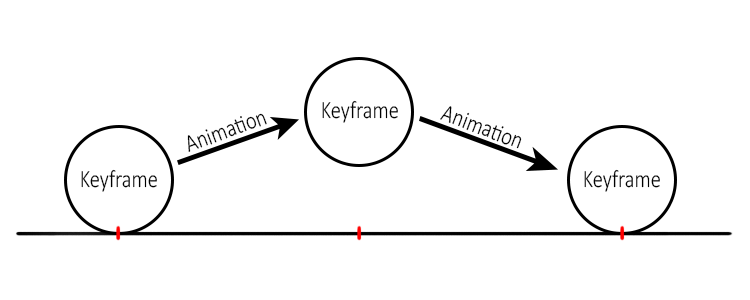
\includegraphics[scale=0.5]{kepek/keyframe_anim.png}
\caption{Kulcsképkocka alapú animáció}
\label{fig:keyframe}
\end{figure}

A vertex alapú animációt a 3D játékfejlesztésben karakterek mozgatásához a 2000-es évek elejéig használták. Megvalósítása egyszerűbb, viszont sok memóriát igényel a tárolása, és nem eredményez olyan természetes mozgást általában, mint a csontváz alapú animáció. Ezt a technológiát többek között a Quake 1, 2 és 3 alkalmazta.

\subsection{Az md2-es formátum}

% TODO: GL\_TRIANGLE\_FAN belelóg a margóba!

Az md2-es modelltárolási formátumot az \textit{idSoftware} fejlesztette ki 1997-ben a Quake 2 nevű játékához. A formátum kulcsképkocka animációk tárolására alkalmas. Tartalmazza az adott modell geometriáit, és a képkockánkénti animációkat. A fájl adatai olyan struktúrában helyezkednek el, hogy könnyedén kirajzoltatható legyen a \texttt{GL\_TRIANGLE\_FAN} és \texttt{GL\_TRIANGLE\_STRIP} OpenGL függvényekkel. A formátum két fő részből áll: fejlécből és adatrészből. A fájl nem tartalmazza a modellek textúráját.

A fejléc egy struktúra, amely a fájl elején kezdődik, és tartalmazza az összes, feldolgozás szempontjából lényeges információt a fájl egészéről. Ilyen például a textúra szélessége, magassága, egy képkocka mérete, képkockák száma.

\section{Csontváz alapú animáció}

A legtöbb mai játék ezt a módszert alkalmazza karakterek mozgatásához. Az alapötlete az, hogy a mozgatható részeket hierarchiába szervezi. Az élőlények felépítése általában olyan, hogy ezzel a fajta animálási móddal egyszerűen modellezhetők. 

A csontváz alapú animáció kapcsolódási pontokból (\textit{joint}-okból) építkezik. Ember esetén például a kézfej kapcsolatban van az alkarral, az alkar a felkarral, ami pedig a test többi részével. Minden hajlási pont egy új kapcsolódási pontot jelent. Tehát ha az ember felkarját megmozdítjuk, mozdul vele a kezének a többi része is. Ezt szemlélteti \aref{fig:skeletal}. ábra.

\begin{figure}[h]
\centering
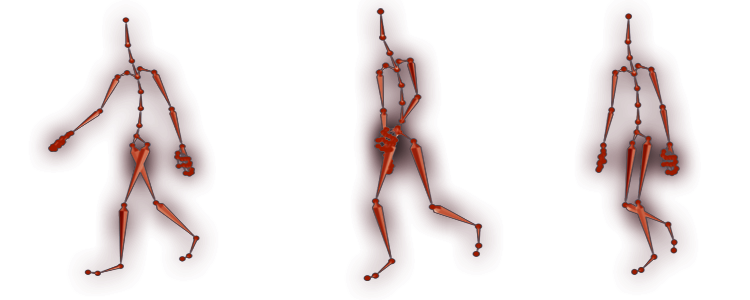
\includegraphics[scale=0.5]{kepek/skeletal_anim.png}
\caption[]{Testrészek hierarchikus kapcsolódási pontjai emberen\footnotemark}
\label{fig:skeletal}
\end{figure}

\footnotetext{forrás: https://www.openflipper.org/media/plugin\_images/skeletalAnimation.png}

Szerencsére a módszer nem csak élőlények modellezésére alkalmazható hatékonyan. A naprendszerünk szintén modellezhető ilyen módon. Vannak a naprendszerünk bolygói, amelyek a tengelyük, és a központi csillag, a Nap körül is forognak.

Előnye, hogy könnyen létre lehet így hozni dinamikus animációkat, mivel az összes karakter csontjait lehet forgatni, mozgatni, továbbá megkönnyíti a bonyolultabb animációk elkészítését. Hátránya viszont, hogy komplexebbek, így több processzoridőt igényelnek.

\subsection{Program: Animáció}

Ennek a programnak az a célja, hogy bemutasson egy animációs módszert, amelyet bárki fel tud használni karakteranimációhoz játékfejlesztésnél. Az animációt megvalósító algoritmus hasznos lehet még egy automatizált gyártósor robotkarjainak mozgatásához is olyan esetekben, amikor például két vagy több karnak mindig egy adott szög tartása mellett, összehangolva kell mozogniuk. A \texttt{Character} osztályban az összes mozgatással és azok pontos megjelenítésével kapcsolatos számítások találhatók. Az \texttt{Action} az állapotok kezeléséért, a \texttt{ModelLoader} és a \texttt{VboDrawer} a modellek (testrészek) betöltéséért, kirajzolásáért felelős, amelyeket a \texttt{MainGame} osztály fog össze. A konkrét felépítés \aref{fig:anim_uml} ábrán látható.

\begin{figure}[h]
\centering
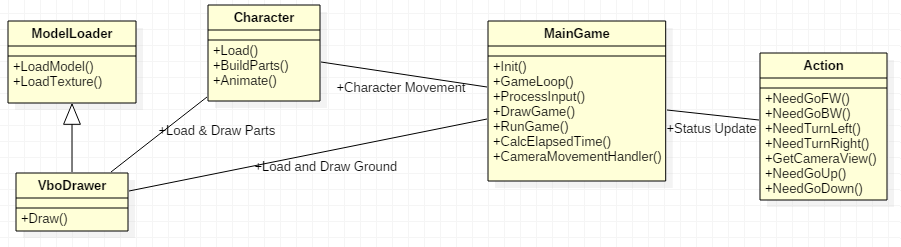
\includegraphics[scale=0.6]{kepek/animation_uml.png}
\caption[]{Az animációt bemutató demó felépítése}
\label{fig:anim_uml}
\end{figure}

\Aref{fig:anim_demo} ábrán látható, futó programban egy egyszerű robotot tudunk irányítani, illetve ha a kamerát szabad mozgás módba váltjuk, meg tudjuk tekinteni a testrészek hierarchikus mozgását több szögből is. A robot részei több .obj kiterjesztésű modellből vannak betöltve, amelyek azért vannak külön modellbe tárolva, hogy egymástól függetlenül tudjuk őket mozgatni, ne csak egyben a teljes robotot. A törzshöz csatlakozik a fej, a két kéz, és a két láb. Utóbbi kettő mindig 60 fokos szögkülönbséggel rendelkezik, és ha elérik a maximális, előre megadott kitérési értéket, a mozgás iránya megfordul. Az elérni kívánt mozgásmechanika implementálása után, meg kell adnunk a testrészek pozícióját. A \texttt{Character} oszályban lévő \textsl{BuildParts()} függvény a \texttt{ModelLoader} és a \texttt{VboDrawer} által betöltött és kirajzolt részek megfelelő pozícióba való elhelyezéséért felel, hogy azok egy egész robottá álljanak össze.

Járás közben az adott karakter előre is halad, illetve minimálisan fel és lefelé is mozog a járásból adódóan, és a testrészek fix szögben való mozgatásán kívül definiálnunk kell ezeket is. Figyelni kell, és számításba kell venni azt a jelenséget is, hogy járás közben egy élő ember  földre leért lába fix, azzal lendíti előre magát, így a láb végéhez képest kell megadnunk a hierarchiában feljebb lévő testrészek mozgását is, ezt nevezzük inverz kinematikának. Az előre és a fel-le irányba való mozgást a következő összefüggéssel írhatjuk fel:
$$
\Delta f = \left|
d \cdot \sin(\alpha)
\right|, \quad u = d \cdot \cos(\alpha),
$$

ahol $\Delta f$ az időegység alatt megtett előre mozgásnak a mértéke (\textit{forward}), az $u$ pedig a karakter fel-le mozgásának animálásához szükséges érték (\textit{up}). A $d$ az egységnyi idő alatt megtett távolságot jelöli (\textit{distance}), az $\alpha$ pedig a jobbláb animálásánál figyelembe vett szög értéke.

Az animálásért felelős részek időfüggőek, ugyanis garantálni kell hogy a különböző teljesítményű gépeken ugyanolyan gyors legyen az animáció. A két kirajzolt képkocka közötti eltelt időt a \texttt{CalcElapsedTime} függvény számolja, amelynek a kimeneti értéke az $s = v \cdot t$ képlettel számolható, ahol $s$ a megtett út, $v$ a sebesség, $t$ pedig az eltelt idő. Minél több a másodpercenként megjelenített képkockák száma, annál kisebb a köztük eltelt idő, és a mozgást annál kisebb értékkel szorozza be, így minden esetben ugyanolyan gyorsan fog mozogni az objektumunk, csak az animáció folytonosságában lesz különbség.

\begin{figure}[h]
\centering
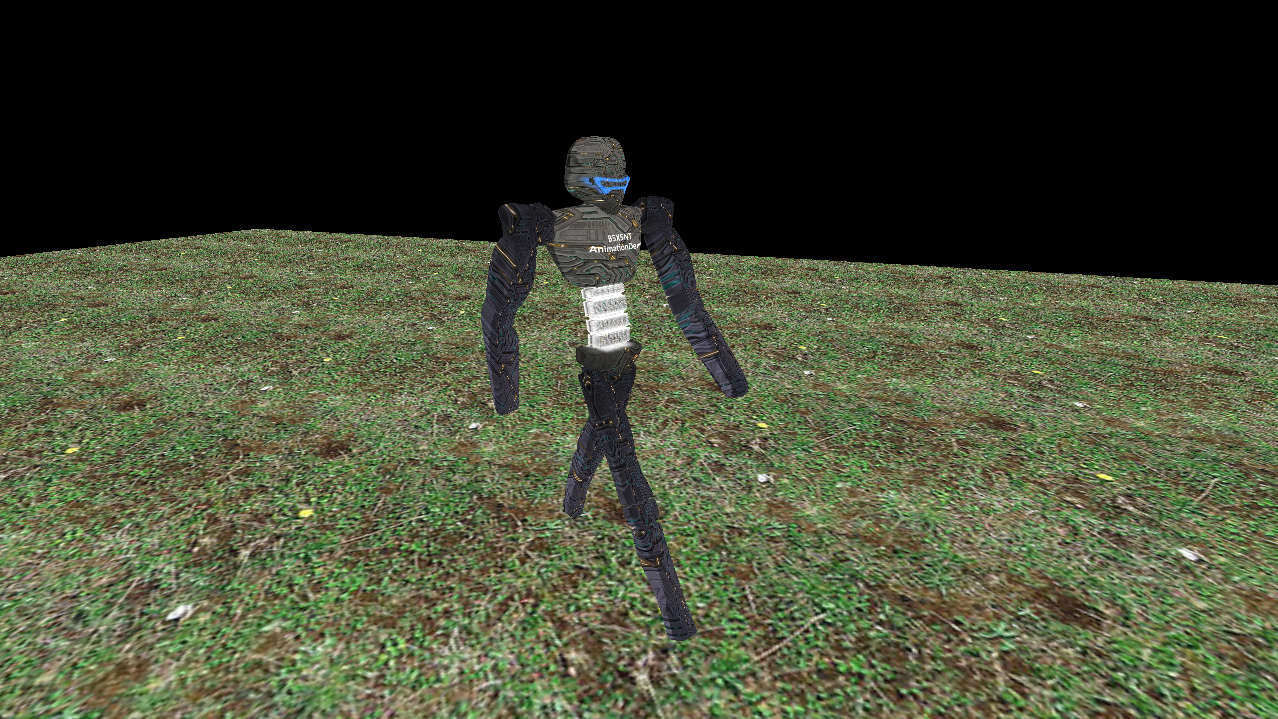
\includegraphics[scale=0.4]{kepek/animation_demo.png}
\caption[]{Pillanatkép az animációt bemutató demóból}
\label{fig:anim_demo}
\end{figure}

A kamera alapesetben a robot mögött van, és annak mozgását követi, amelyet szintén a felhasználó tud irányítani. Az animáció bármikor félbeszakítható, nem áll vissza az alapértelmezett állásba, hogy megtekinthető legyen a mozgás minden fázisa.

\section{Interpolációs módszerek}

% Interpoláció: https://hu.wikipedia.org/wiki/Interpol%C3%A1ci%C3%B3#Lagrange-interpol.C3.A1ci.C3.B3

Animációkészítés során többféle interpolációt használhatunk, ami azt jelenti, hogy ismert értékek alapján, a közbülső pontokra, vagyis nem ismert értékekre adunk közelítést.

Különféle interpolációs módszerek vannak. A választás közülük nyilván attól függ, hogy pontosan mit szeretnénk megvalósítani. Egyszerűbb esetekben még megfelelő a lineáris interpoláció, viszont általában túlságosan szögletes mozgást eredményez, ezért valamilyen simább görbével való útvonal közelítést érdemes használni.

\subsection{Lineáris interpoláció}

Ez a legegyszerűbb interpolációs módszer, minden pontot egy egyenessel kötünk össze. Nem összetett mozgásoknál ez megfelelő lehet, viszont ha több mozgás követi egymást rögtön, akkor darabos. Minden előre meghatározott pont, amit érinteni kell egy törést jelent, így komplexebb, sima mozgásokhoz nem alkalmas, ez látható \aref{fig:linear}. ábrán.

\begin{figure}[h]
\centering
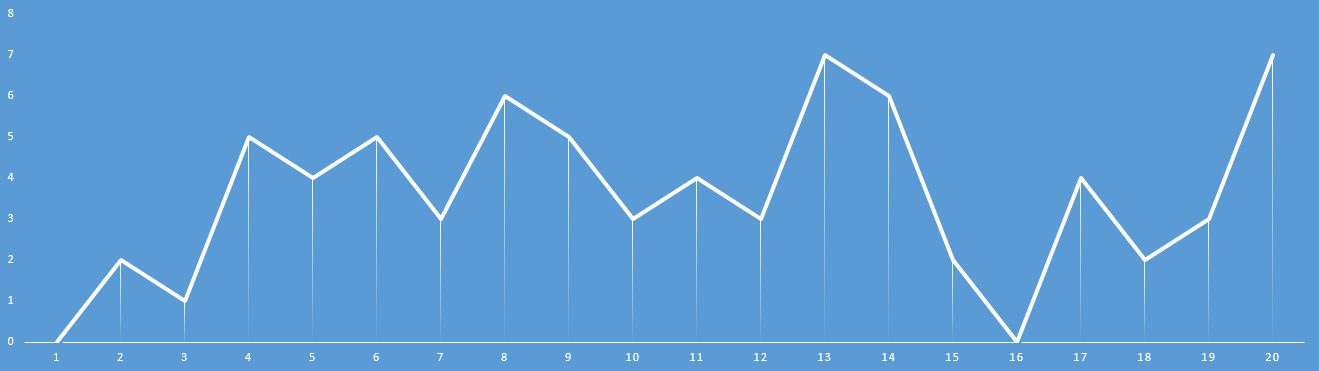
\includegraphics[scale=0.43]{kepek/linear_interpol.png}
\caption{Lineáris interpoláció}
\label{fig:linear}
\end{figure}

\subsection{Lagrange-interpoláció}

Mivel a függvény sima, deriváltja folyontos, sokkal életszerűbb megközelítést lehet elérni vele, mint a lineáris interpolációval. Viszont nagy hátránya, hogy egyes esetekben indokolatlanul nagy hullámzások jelenhetnek meg a kirajzolt függvényen, közvetlen egymás mellett lévő két pont között, ez látható \aref{fig:lagrange}-es ábrán. Így ez az interpoláció animációhoz nem minden esetben alkalmas.

\begin{figure}[h]
\centering
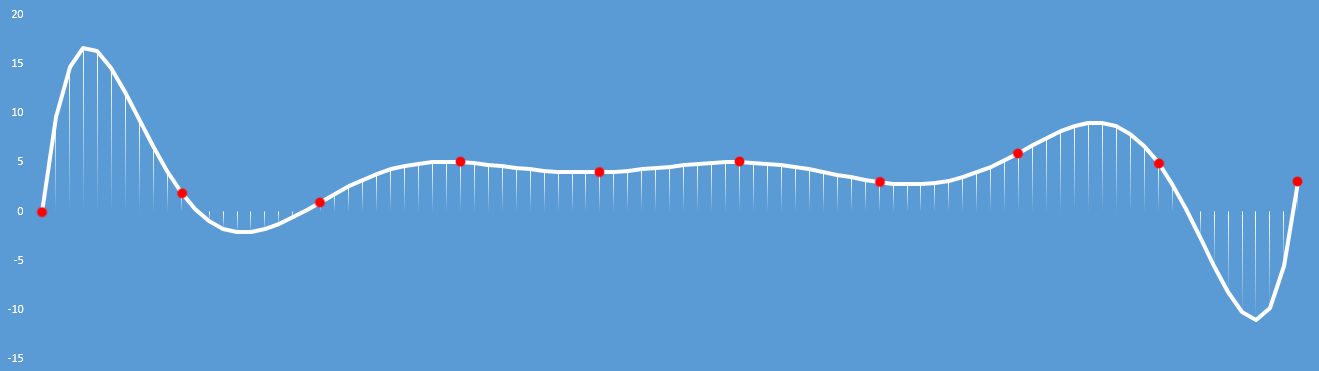
\includegraphics[scale=0.43]{kepek/non_linear_interpol.png}
\caption{Lagrange-interpoláció}
\label{fig:lagrange}
\end{figure}

\subsection{B-spline}

Komplexebb animációknál, mint például egy élőlény mozgása, ha nem szeretnénk darabos animációt, akkor a B-spline interpolációt is alkalmazhatjuk. Ez esetben a görbe lokálisan vezérelhető, és a lineáris interpolációval ellentétben nem töredezett, így ez a legalkalmasabb folyamatos animációra. A lokális vezérelhetőség adja az előnyét a Lagrange-interpolációval szemben, mert így nem lehetnek kiugró értékek a grafikus képében.

\subsection{Program: Lagrange Interpoláció}

A felhasználónak lehetősége van megadni, hogy hány darab pontot szeretne definiálni, majd a pontok konkrét $x$ és $y$ koordinátáit, amelyekhez a program kiszámolja az y koordinátát Lagrange-interpolációval. Ez a program azért készült, hogy bemutassa, hogyan működik ez a fajta interpolálás.
Adott két tömb, amelyek tartalmazzák a függvény megadott pontjainak x és y értékeit. A num a tömbök elemeinek számát, az input pedig a bevitt értéket takarja.

\begin{algorithm}[H]
 \KwData{x[]; y[]; num; input; s; t; eredmeny\;}
 \KwResult{Adott x-hez tartozó y koordináta}
\For{i := 0; i < num; i++}{
	s := 1, t := 1\;
	\For{j := 0; j < num; j++}{	
	\If{j != i}{
   		s := s * (input - x[j]);\\
		t := t * (x[i] - x[j])\;
   		}
	}
	eredmeny := eredmeny + ((s / t) * y[i])\;
 }
 \caption{Lagrange-interpoláció implementálása}
\end{algorithm} 

A függvény grafikus megjelenítése az OpenGL-el lett megvalósítva. Az ablak alapértelmezett felbontása 1280x720, amelyhez a bevitt értékeket a program felskálázza úgy, hogy a függvény még sehol sem lógjon ki az ablakból, de a lehető legnagyobb méretű legyen. A skálázás mértékét mind konzolban, mind grafikusan megjeleníti, utóbbit csak addig, míg a szorzó nagyobb mint 9. Ez alatt az osztás már olyan sűrű 1280x720-as felbontás mellett, hogy értelmetlen, és csúnya a grafikus kirajzolása. 
\newpage
A függvény kezdete a legkisebb, a vége pedig a legnagyobb $x$ értéknél van, a köztes részen pedig minden egész $x$-hez kiszámolja a hozzá tartozó $y$-t, majd azokat vonallal összeköti. A konzol eredményei \aref{fig:lagrange_imp}. ábrán, a grafikus megjelenítés pedig \aref{fig:lagrange_demo}. ábrán látható.

\begin{figure}[h]
\centering
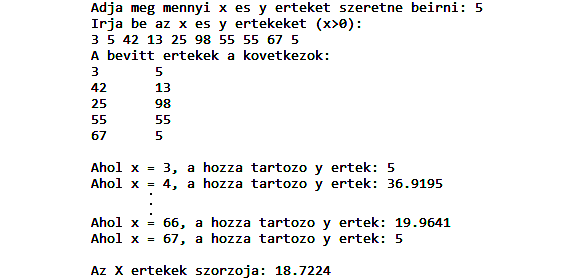
\includegraphics[scale=0.9]{kepek/lagrange_imp.png}
\caption{Lagrange-interpolációs demó}
\label{fig:lagrange_imp}
\end{figure}

\begin{figure}[h]
\centering
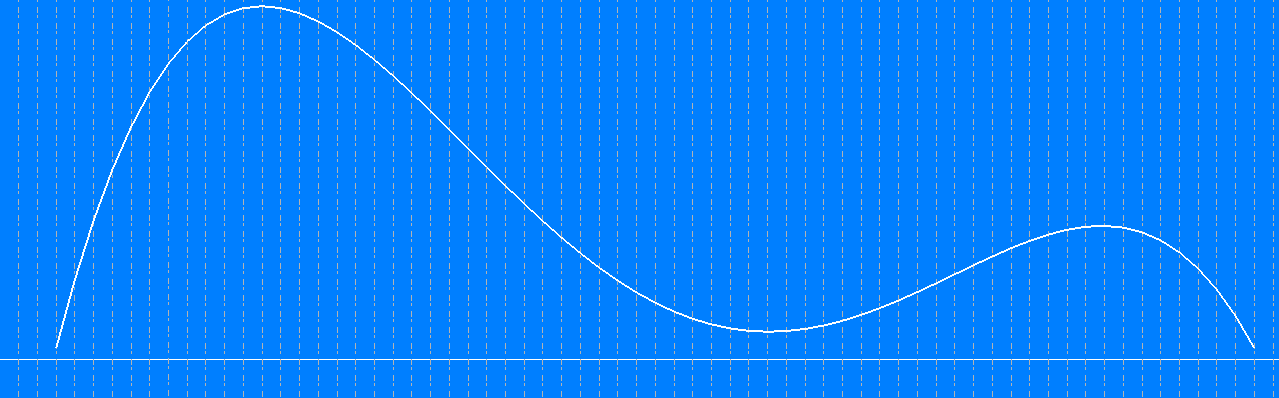
\includegraphics[scale=0.43]{kepek/lagrange_graphics.png}
\caption{Lagrange-interpolációs demó}
\label{fig:lagrange_demo}
\end{figure}

